% cSpell: disable
% !TeX spellcheck = fr-classique
% LTeX: language=fr
\documentclass[aspectratio=169,xcolor=dvipsnames]{beamer}
\usetheme{SimplePlus}

\usepackage{tikz}
\usetikzlibrary{tikzmark}
\usetikzlibrary{decorations.pathreplacing}
\usetikzlibrary{svg.path}
\usetikzlibrary{calc,fit,shapes}
\usetikzlibrary{arrows,chains}
\usetikzlibrary{overlay-beamer-styles}
\usetikzlibrary{shapes.arrows}
\usetikzlibrary{decorations.pathmorphing}

\title{Reseaux de neurones avances pour la reconstruction d'images IRM a partir de donnees fortement sous-echantillonees dans des contextes d'acquisition difficiles.}
\subtitle{MT180}

\titlegraphic{
    \begin{tikzpicture}[overlay,remember picture]
        \node[below right=0.2cm and 0.2cm of current page.150] (cea) {
\includegraphics[width=4em]{Figures/logos/CEA_logo.jpg}};
        \node[right=of cea] (neurospin) {
\includegraphics[width=4em]{Figures/logos/neurospin_logo.jpg}};
        \node[right=of neurospin] (cosmostat) {
\includegraphics[width=6em]{Figures/logos/cosmostat_logo.jpg}};
        \node[right=of cosmostat] (inria) {
\includegraphics[width=6em]{Figures/logos/inria_logo.jpg}};
        \node[right=of inria] (parietal) {
\includegraphics[width=6em]{Figures/logos/parietal_logo.jpg}};
    \end{tikzpicture}
}

\author[Zaccharie] {Zaccharie Ramzi \\  {\footnotesize directeurs: Philippe Ciuciu et Jean-Luc Starck}}
\institute[Inria-CEA] % Your institution as it will appear on the bottom of every slide, may be shorthand to save space
{
    Equipe Parietal, Inria Saclay \\
    NeuroSpin et Cosmostat, CEA Saclay
}

\begin{document}

\begin{frame}
    % Print the title page as the first slide
    \titlepage
\end{frame}

{
\usebackgroundtemplate{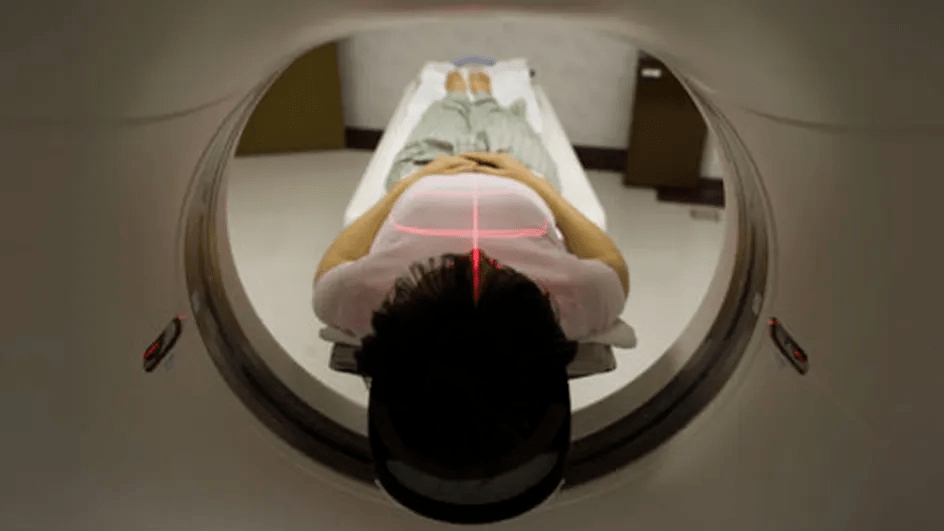
\includegraphics[width=\paperwidth]{Figures/inside_mri.png}}
\def\clockradius{4.3cm}
\definecolor{cadmiumred}{rgb}{0.89, 0.0, 0.13}
\begin{frame}[plain]
      \begin{center}
        \begin{tikzpicture}[line cap=rect,line width=3pt,color=cadmiumred,opacity=0.6]
            \draw (0,0cm) circle [radius=\clockradius];
            \foreach \angle [count=\xi] in {60,30,...,-270}
            {
              \draw[line width=1pt] (\angle:\clockradius-0.2cm) -- (\angle:\clockradius);
              \node[font=\large] at (\angle:\clockradius-0.64cm) {\textsf{\xi}};
            }
            \foreach \angle in {0,90,180,270}
              \draw[line width=2pt] (\angle:\clockradius-0.4cm) -- (\angle:\clockradius);
            \draw (0,0) -- (120:2.4cm);
            \draw (0,0) -- (90:3cm);
            \end{tikzpicture}
      \end{center}
\end{frame}
}

\end{document}